%!TEX root =presentation.tex
\section[godunov]{Godunov discretization} % (fold)
\label{sec:godunov_discretization}

\subsection{Discretizing single system} % (fold)
\label{sub:discretizing_single_system}

% subsection discretizing_single_system (end)

\begin{frame}
\frametitle{Discretizing via Godunov method}

\begin{itemize}
    \item Cannot represent (or not practical to represent) continuous function on computer.
    \item Approximate solution by discretizing space and time.
    \item Solve for vector of discrete variables.
\end{itemize}

\begin{block}{Godunov's scheme (high level)}
\begin{enumerate}
    \item Split system in discrete chunks of size $\Delta x$.
    \item Approximate IC by averaging over $\Delta x$.
    \item Find exact sln of system by solving Riemann problems at discretized boundaries for $\Delta t$ time.
    \item Approximate new sln by averaging over $\Delta x$.
    \item Set IC as new sln and go to step 3.
\end{enumerate}
\end{block}

\end{frame}

\begin{frame}



\begin{figure}
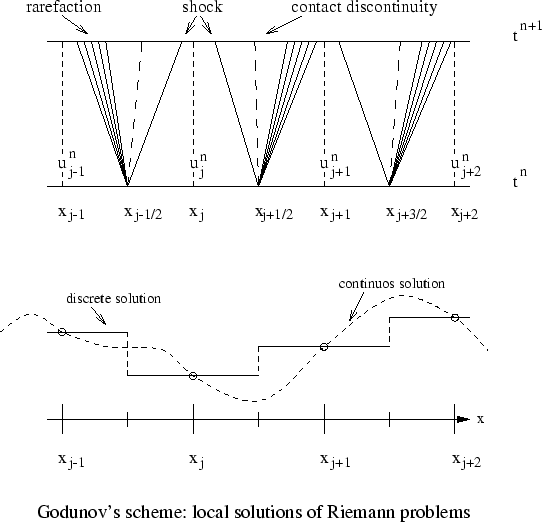
\includegraphics[width=.65\columnwidth]{images/godunov}
\caption{credit: http://www.uv.es/astrorela/simulacionnumerica/node34.html}
\end{figure}


\end{frame}

\begin{frame}
\frametitle{Derivation of Godunov's method}

Take a discrete initial condition $\initstate^{\Delta}$. We want $\discrete{\xind}{\Delta t}$, the average value at cell ${\xind}$ at time $\Delta t$:

\begin{equation}
\discrete{\xind}{\Delta t}\approxeq\dfrac{1}{\Delta x}\int_{\xdis{\xind-\frac{1}{2}}}^{\xdis{\xind+\frac{1}{2}}}\dvar^{\Delta}(\Delta t,x)dx.
\end{equation}

where $\dvar^{\Delta}(\Delta t,x)$ is an exact solution of the Cauchy problem
with initial condition $\initstate^{\Delta}$.



This requires solution of $\cvar(x,t)$ over $[\xdis{\xind - \frac{1}{2}},\xdis{\xind + \frac{1}{2}}]\times [0,\Delta t]$.

\begin{figure}
\centering
\subfloat[Space discretization for a link $\link\in\links$]{%
      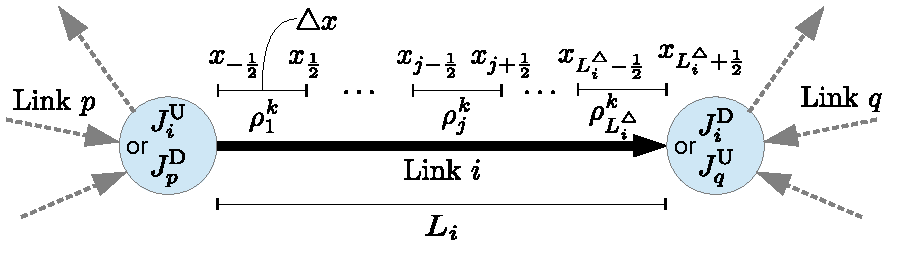
\includegraphics[width=0.8\columnwidth]{../figs-gen/dx}
    }
\end{figure}

\end{frame}
\begin{frame}


But since Riemann problems are self-similar, fluxes across boundaries are constant:

\[
f(\cvar(t,\xdis{\xind + \frac{1}{2}}))=f(W_{R}(0;\discrete{\xind}{\tind},\discrete{\xind+1}{\tind})).
\]

\[
f(\cvar(t,\xdis{\xind-\frac{1}{2}}))=f(W_{R}(0;\discrete{\xind-1}{\tind},\discrete{\xind}{\tind})).
\]

\begin{figure}
\centering
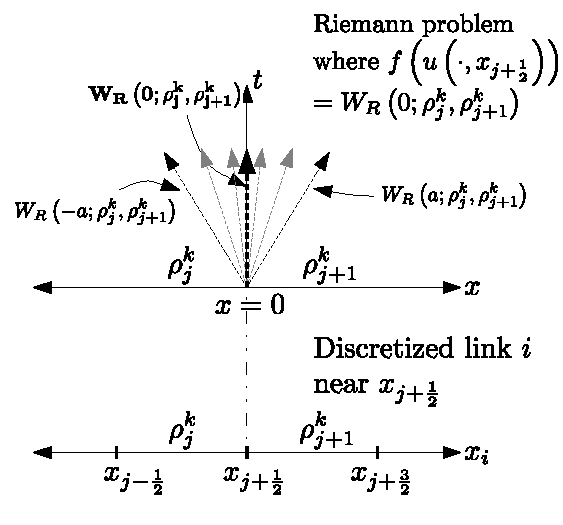
\includegraphics[width=0.5\columnwidth]{../figs-gen/dx-to-riemann}
\end{figure}

% \begin{equation}
%     \int_{0}^{\Delta t}f\left(u\left(t,x_{i}\right)\right)dt\approx\Delta tg^{G}\left(\dvar_{i},\dvar_{i+1}\right)
% \end{equation}

% where $g^G$ is the flux across cell boundaries obtained via sln of Riemann problem.

% Now only function of discrete values:

% \begin{equation}
% \bar{\dvar}_{i}=\dvar_{i}-\frac{\Delta t}{x_{i+1}-x_{i}}\left(g^{G}\left(\dvar_{i},\dvar_{i+1}\right)-g^{G}\left(\dvar_{i-1},\dvar_{i}\right)\right)    
% \end{equation}


\end{frame}

\begin{frame}
    \begin{equation}
\discrete{\xind}{\tind+1}=\discrete{\xind}{\tind}-\frac{\Delta t}{\Delta x}(\god(\discrete{\xind}{\tind},\discrete{\xind+1}{\tind})-\god(\discrete{\xind-1}{\tind},\discrete{\xind}{\tind})),\label{eq:godscheme}
\end{equation}
where $g^{G}$ is the numerical flux:
\[
\god\left(\discrete{\xind}{},\discrete{\xind+1}{}\right)=f(W_{R}(0;\discrete{\xind}{},\discrete{\xind+1}{}))
\]

\textbf{No longer depends on solution of continuous function.}

\begin{figure}
\centering
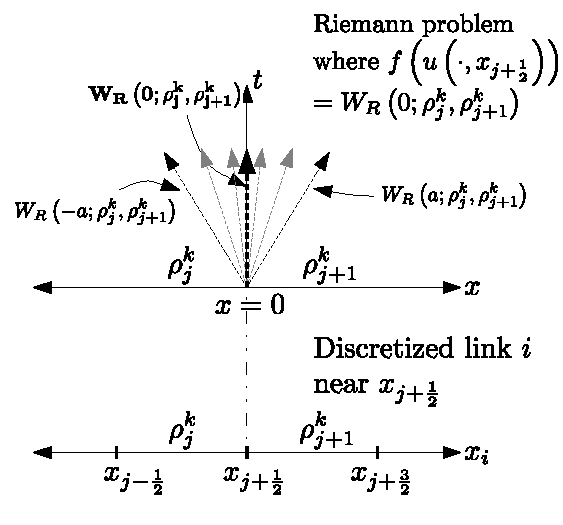
\includegraphics[width=0.45\columnwidth]{../figs-gen/dx-to-riemann}
\end{figure}

\end{frame}

% \begin{frame}[t]\frametitle{CFL condition}

% In previous derivation, it is assumed no solution from one Riemann problem influences another at the discrete boundaries.

% This limits how large the time-step to guarantee convergence of Godunov scheme to continuous solution.

% \begin{block}{The Courant Friedrichs Lewy (CFL) condition}
% \begin{equation}
%     \lambda^{\max}\le\frac{\Delta x}{\Delta t}
% \end{equation}
% \end{block}

% \end{frame}

\subsection{Discretizing PDE network} % (fold)
\label{sub:discretizing_pde_network}

\begin{frame}

Solving for Godunov flux easy for $1$-to-$1$ junctions. What about $n$-to-$m$?

\begin{figure}
\includegraphics<1>[width=\columnwidth]{figs-gen/god-rp}
\includegraphics<2>[width=\columnwidth]{figs-gen/god-rp-sln}
\end{figure}

\begin{itemize}
    \item<2> Apply Riemann solver at junction
    \item<2> Use Riemann solution as boundary condition for $g^G$ at junction.
\end{itemize}

\end{frame}

% \begin{frame}
% \frametitle{Summary of Godunov scheme for PDE networks}


% \begin{enumerate}
% \item<1-> Begin with initial condition ($t=0$) $\left\{ \initstate_{\link}:\link\in\links\right\} $.
% \item<2-> For every junction $\jn\in\jns$:
% \begin{enumerate}
% \item<2-> Apply the Riemann solver to Riemann data to obtain the boundary condition
% $\hat{\mathbf{\dvar}}_{\jn}=$\RS\tuple{\discrete 1{\tind}}{\discrete{\ninc+\nout}{\tind}}$.
% \end{enumerate}
% \item<3-> For every link $\link\in\links$:

% \begin{enumerate}
% \item<3-> Letting $\jn_{\link}^{\text{Up}}=\jn\in\jns:\link\in Out\left(\jn\right)$
% and $\jn_{\link}^{\text{Down}}=\jn\in\jns:\link\in In\left(\jn\right)$,
% the discrete value over link $\link$ at time $\Delta t$, $\bar{\dvar}_{\link}$,
% is given by:
% \end{enumerate}

% \[
% \bar{\dvar}_{\link}=\dvar_{\link}-\frac{\Delta t}{L_{\link}}\left(f\left(\left\{ \mathbf{\hat{\dvar}}_{\jn_{\link}^{\text{Down}}}\right\} _{\link}\right)-f\left(\left\{ \mathbf{\hat{\dvar}}_{\jn_{\link}^{\text{Up}}}\right\} _{\link}\right)\right)
% \]

% \end{enumerate}

% \end{frame}

\begin{frame}
\frametitle{Summary of Godunov scheme for PDE networks}

\begin{algorithm}[H]
\caption{\texttt{Riemann solver update procedure}}
\lstinputlisting[basicstyle={\ttfamily\footnotesize},breaklines=true,label={algo:rs-alg},mathescape=true]{../rs-alg}
\end{algorithm}

\end{frame}

\begin{frame}
\frametitle{Summary of Godunov scheme for PDE networks}

Or by using the flux solution directly...

\begin{algorithm}[H]
\caption{\texttt{Godunov junction flux update procedure}}
\lstinputlisting[basicstyle={\ttfamily\footnotesize},breaklines=true,label={algo:god-alg},mathescape=true]{../god-alg}
\end{algorithm}

\end{frame}

% subsection discretizing_pde_network (end)

% section godunov_discretization (end)